\lab{Applications}{Projectile Tracking}{Projectile Tracking}
\objective{Understand how to use a Kalman filter for projectile tracking}

Suppose that a projectile, say, an artillery round, is launched, and as it passes by a radar sensor we are able to take noisy measurements of its position (but not its velocity). We would like to smooth out those noisy estimates and predict the point of impact and the point of origin. We will use this with a Kalman filter, using the laws of physics to help us formulate our system models.

We can consider the state of the projectile to be its position and its velocity. Considering this projectile to be traveling through $\mathbb{R}^{2}$, both the position and velocity have horizontal and vertical components, so we can write the state of the projectile as 
\begin{equation*}
\mathbf{x} = \left( \begin{array}{c} s_{x} \\ s_{y} \\ v_{x} \\ v_{y} \end{array} \right)
\end{equation*}

We consider the system to evolve in discrete time steps, according to $$\mathbf{x}_{k+1} = F\mathbf{x}_{k} + \mathbf{u} + \mathbf{w}_{k}.$$

\begin{problem}
Using a discrete time step of $0.1$ seconds, and considering the standard gravitational acceleration of $-9.8 \frac{m}{s}$, determine a matrix $F$ and control vector $\mathbf{u}$ to describe this process. You may assume the projectile experiences no drag. Further assuming 
\begin{align*}
H & = \left( \begin{array}{cccc} 1 & 0 & 0 & 0 \\ 0 & 1 & 0 & 0 \end{array} \right) \\
Q & = 0.1 \cdot I_{4} \\
R & = 500 \cdot I_{2}
\end{align*}
and an initial system state 
\begin{equation*}
\mathbf{x}_{0} = \left( \begin{array}{c} 0 \\ 0 \\ 300 \\ 600 \end{array} \right)
\end{equation*}
evolve the system forward until the projectile hits the ground again. We should have approximately $1200$ states $\mathbf{x}_{k}$ and $1200$ measurements $\mathbf{z}_{k}$.
\end{problem}

We now assume that our radar sensor can only detect the projectile from time step $200$ to $800$.

\begin{problem}
Plot the entire projectile path as a smooth blue curve, and plot the measurements from time step $200$ to $800$ as red points. Zoom in so you can see the inaccuracies caused by measurement noise. Your plots should be similar to Figure \ref{fig:problem2}, though you do not have to zoom in on the same region.
\end{problem}

\begin{figure}
	\centering
	\begin{tabular}{cc} 
	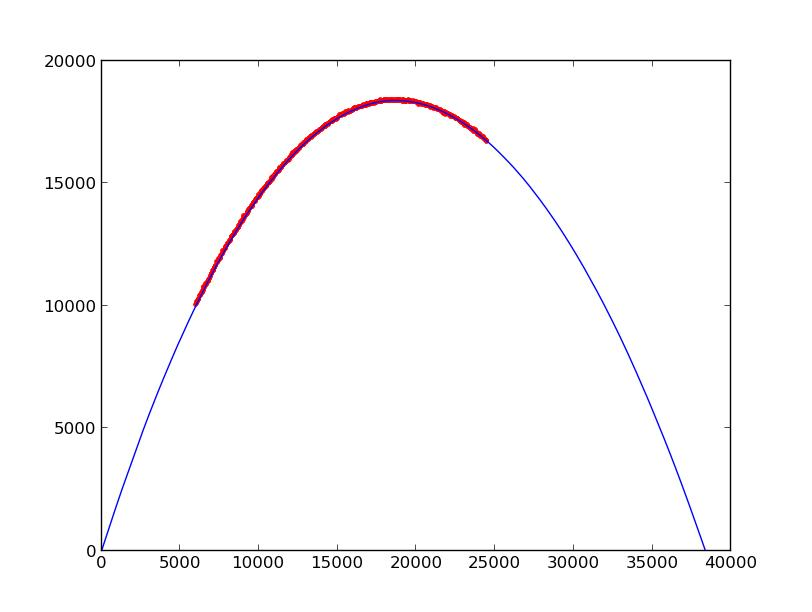
\includegraphics[width=.49\textwidth]{problem2_1.jpg} & 
	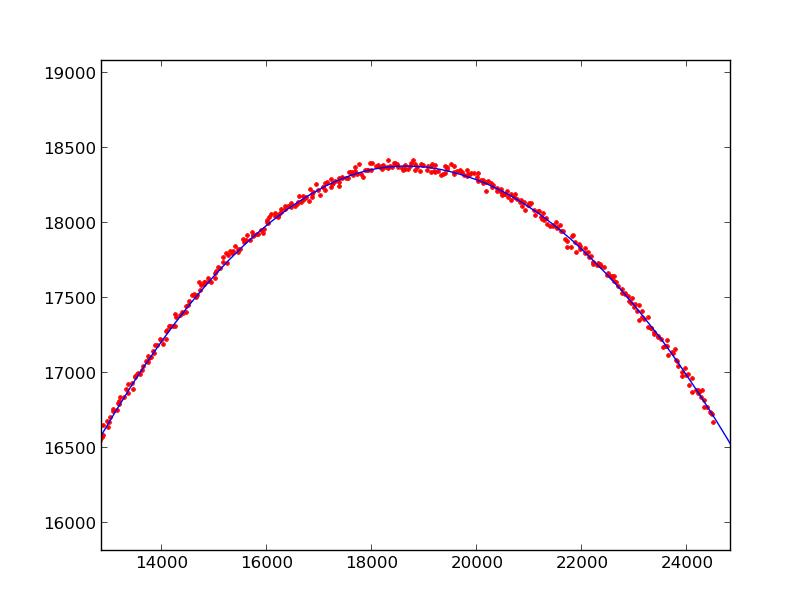
\includegraphics[width=.49\textwidth]{problem2_2.jpg}
	\end{tabular}
	\caption{Projectile path and noisy measurements}
	\label{fig:problem2}
\end{figure}

Because we cannot detect the true states, we would like to estimate them between time step $200$ and $800$ using a Kalman filter and the measured observations.

\begin{problem}
Initialize the Kalman filter at time step $200$. Use the measured position at time $200$ and compute the average velocity from the first $10$ position measurements. Use these estimates as your initial state estimation $\widehat{\mathbf{x}}_{200}$. Using $P_{200} = 10^{6} \cdot Q$ and your Kalman filter, compute the next $600$ state estimates. Plot these state estimates as a smooth green curve along with your previous plot. Zoom in to see how well it follows the true path. Your plots should be similar to Figure \ref{fig:problem3}.
\end{problem}

\begin{figure}
	\centering
	\begin{tabular}{cc} 
	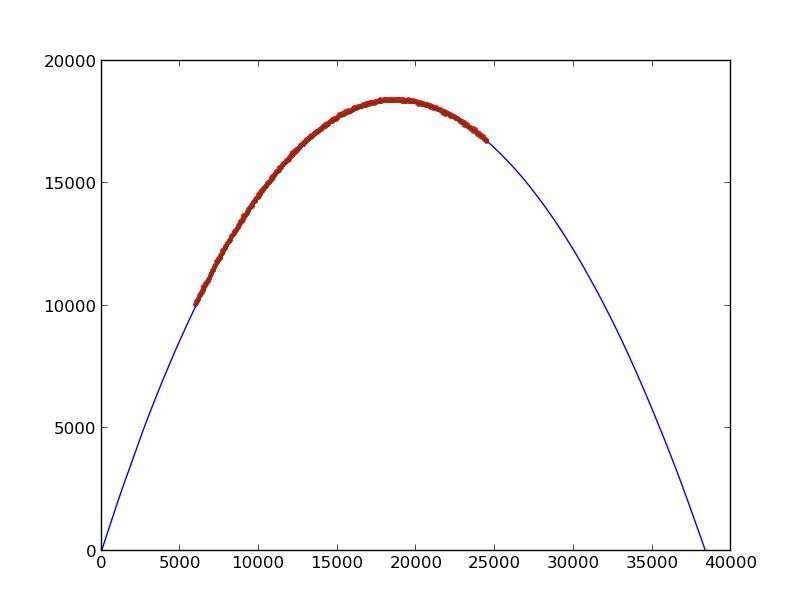
\includegraphics[width=.49\textwidth]{problem3_1.jpg} & 
	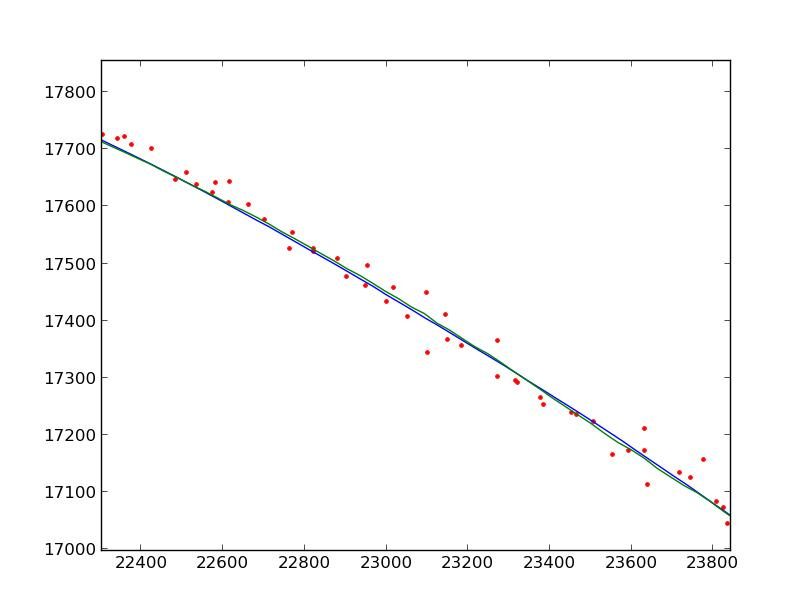
\includegraphics[width=.49\textwidth]{problem3_2.jpg}
	\end{tabular}
	\caption{State estimation curve}
	\label{fig:problem3}
\end{figure}

We would like to know if the projectile is going to hit us, so we want to predict the point of impact.

\begin{problem}
Using your final state estimate $\widehat{\mathbf{x}}_{800}$, predict the position of the projectile at each time step up until impact. Plot this path as a smooth yellow curve along with your previous plots. Zoom in to see how accurate your prediction is. Your plots should be similar to Figure \ref{fig:problem4}.
\end{problem}

\begin{figure}
	\centering
	\begin{tabular}{cc} 
	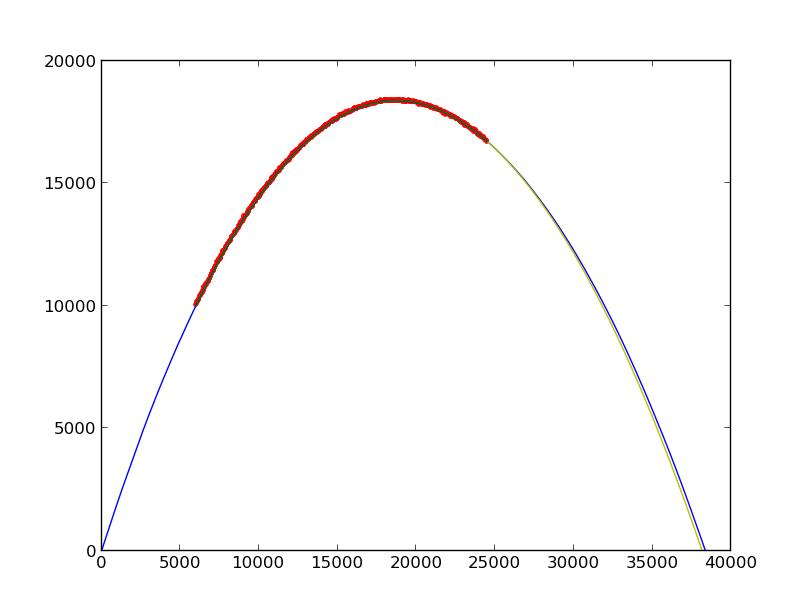
\includegraphics[width=.49\textwidth]{problem4_1.jpg} & 
	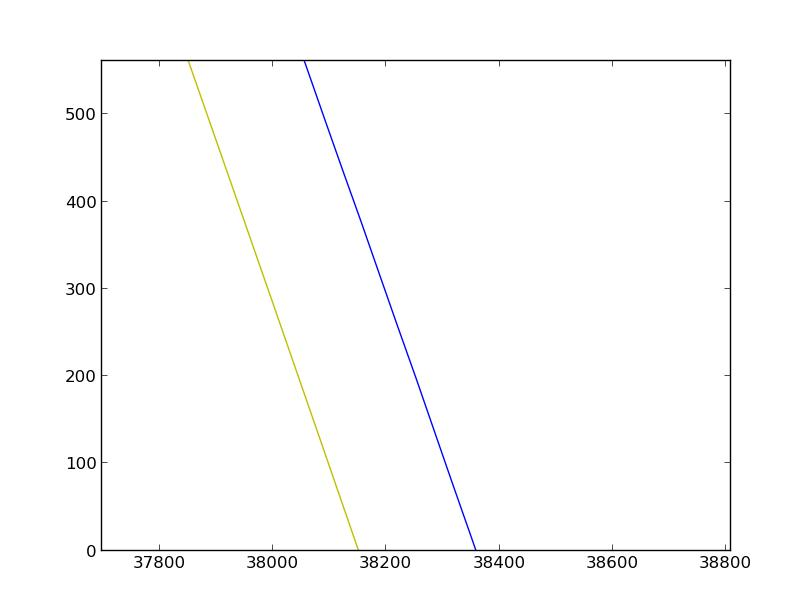
\includegraphics[width=.49\textwidth]{problem4_2.jpg}
	\end{tabular}
	\caption{Point of impact}
	\label{fig:problem4}
\end{figure}

Now that we have moved out of the way, we would like to return fire to whoever launched the projectile. Thus we need to predict the point of origin.

\begin{problem}
Using your state estimate $\widehat{\mathbf{x}}_{250}$, predict the point of origin using the reversed system from the previous lab. Plot the estimated position of the projectile from time step $0$ up through time step $250$ as a smooth cyan curve. Zoom in to see how accurate your prediction about the point of origin is. Your plots should be similar to Figure \ref{fig:problem5}.
\end{problem}

\begin{figure}
	\centering
	\begin{tabular}{cc} 
	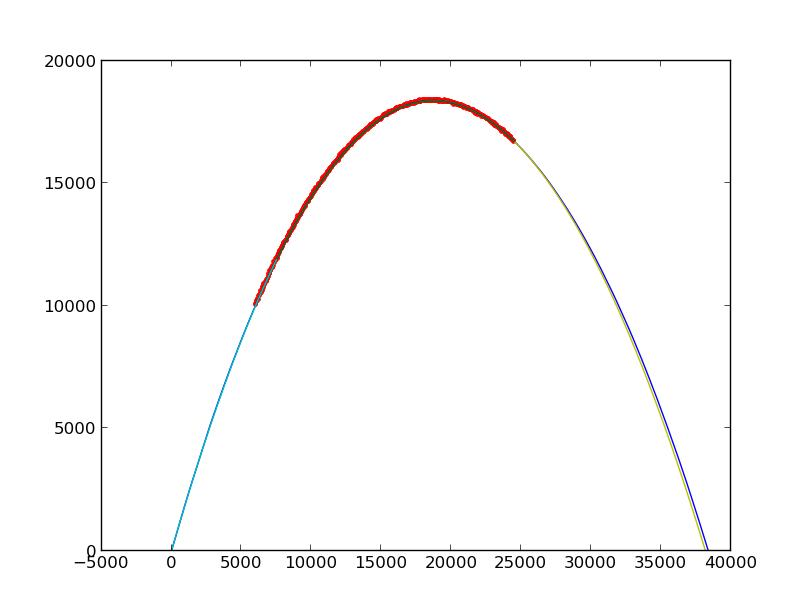
\includegraphics[width=.49\textwidth]{problem5_1.jpg} & 
	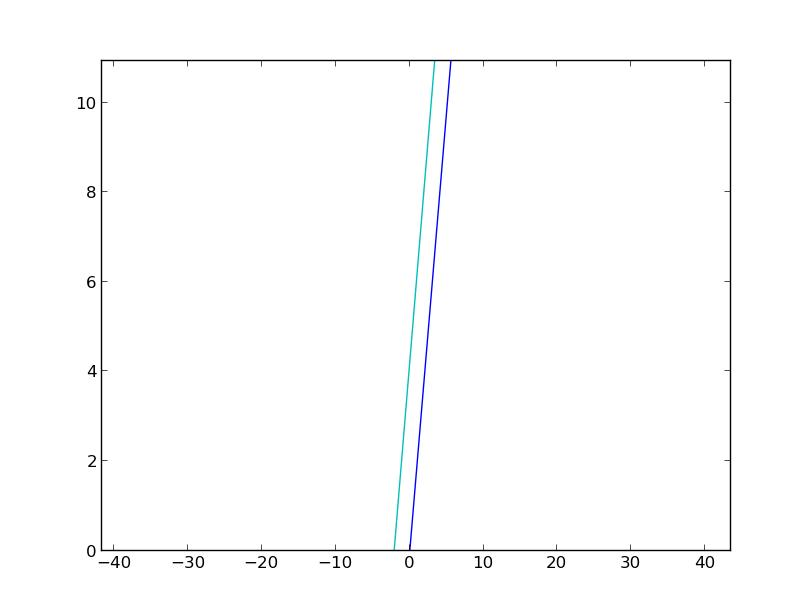
\includegraphics[width=.49\textwidth]{problem5_2.jpg}
	\end{tabular}
	\caption{Point of origin}
	\label{fig:problem5}
\end{figure}